%
% ---- Technologies
%

\section{Conclusion and Future Work}

...

An interesting area of future work might be in using the modelling techniques in adaptive algorithms.  A model might be used as a policy for elastic scaling, and compared with the performance of other right-sizing strategies; control theory, machine learning and other model based techniques including statistical.

%
% ---- Operational microservices
%
\subsection{Operational microservices}

A more `natural' microservices architecture partitions the system by operation (Book, Search, Return) with a separate database for each.  The databases maintain eventual consistency via an event streaming application e.g. using Kafka.
\begin{enumerate}
\item Book is an event producer and consumer (produces when a ticket is booked, consumes returned tickets).
\item Search is an event consumer (consumes the state of tickets that are booked and returned).
\item Return is an event producer (produces returned tickets).
\end{enumerate}

\begin{figure}
	\caption{Operational microservices architecture}
	\centering
	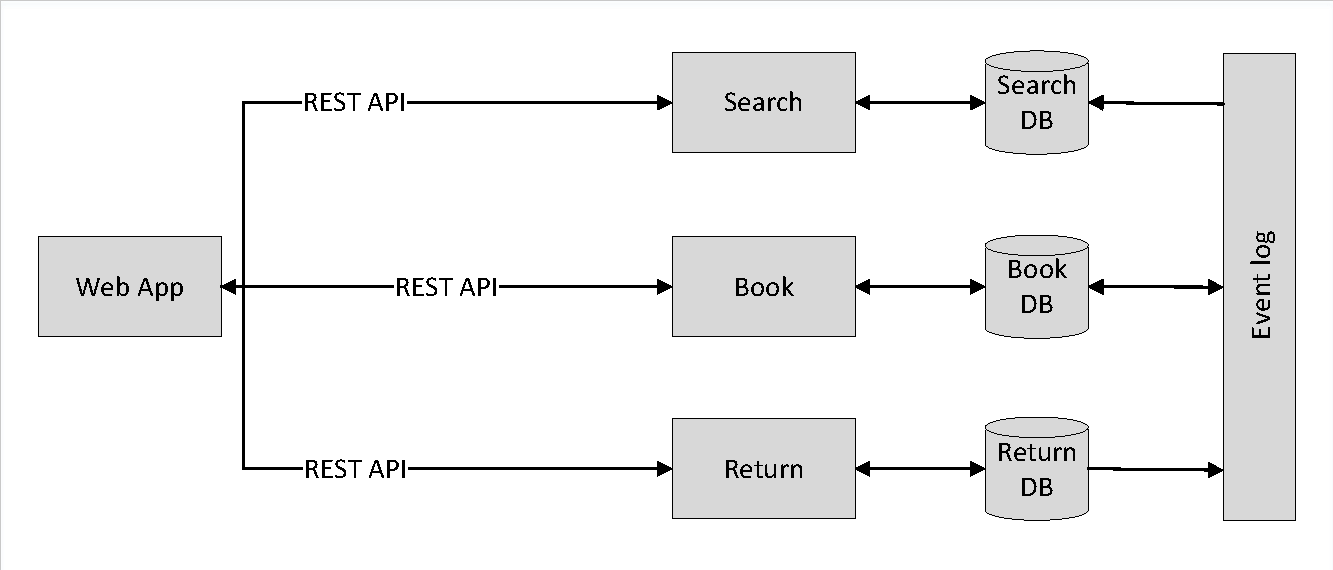
\includegraphics[trim = 5 5 5 5, clip, width=\textwidth]{img/operationmicro}
\end{figure}